\chapter{Oberflächen}
Im Nachfolgendem werden die Benutzeroberflächen der Applikation, die enthaltenen Bedienelemente und deren jeweilige Funktion beschrieben.
\section{Authentifizierung}
Zu Beginn einer Sitzung muss sich jeder Anwender -- unabhängig von seiner Rolle -- mit seiner E-Mailadresse und dem zugehörigem Passwort anmelden. 
Es sind nur E-Mailadressen der Hochschule Landshut zulässig.
Die Bedienungsoberfläche für den ersten Benutzungsschritt wird in Abbildung \ref{pic:ActivityLogin} dargestellt.
Im Feld \enquote{Email} wird die Mailadresssee des Anwenders und analog dazu im Feld \enquote{Passwort} das Passwort eingetragen.
Durch Klick auf den Knopf \enquote{Sign In} startet ein Authentifizierungsversuch.
Zunächst überprüft die Applikation die syntaktische Korrektheit der Mailadresse und informiert gegebenenfalls über ungültige Eingaben.
Im Falle einer validen Eingabe werden die Anmeldedaten an den Server geleitet und mit der Datenbank abgeglichen.
Existiert ein Benutzer mit den jeweiligen Daten, so wird die zugeordnete Rolle übermittelt.
Abhängig von der Antwort des Servers öffnet sich dann die Oberfläche \enquote{\nameref{section:DozentenOberflache}} oder 
\enquote{\nameref{section:StudentenOberflache}}.

\begin{figure}[H]
	\begin{center}
	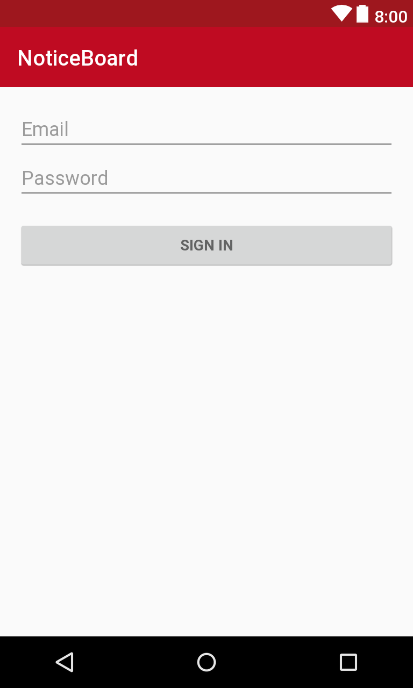
\includegraphics[scale=0.15]{Resources/ActivityLogin}
	\caption{Oberfläche für das Anmelden in der Applikation}
	\label{pic:ActivityLogin}
	\end{center}
\end{figure}

\section{Oberfläche für Dozenten}\label{section:DozentenOberflache}
Hat sich ein Nutzer der Rolle \enquote{Dozent} erfolgreich angemeldet, so erscheint die Oberfläche \enquote{MyClassrooms}.
Hier werden alle Klassenräume angezeigt, die er verwaltet.
Der Dozent hat nun die Möglichkeit entweder über den Button mit dem Löschen-Symbol Klassenräume und alle enthaltenen Nachrichten zu löschen (siehe Abbildung \ref{pic:LecturerDeleteClassroom}) oder über den Button unten Rechts einen neuen Klassenraum zu erstellen (siehe Abbildung \ref{pic:LecturerCreateClassroom}). 

\begin{figure}[H]
	\begin{center}
	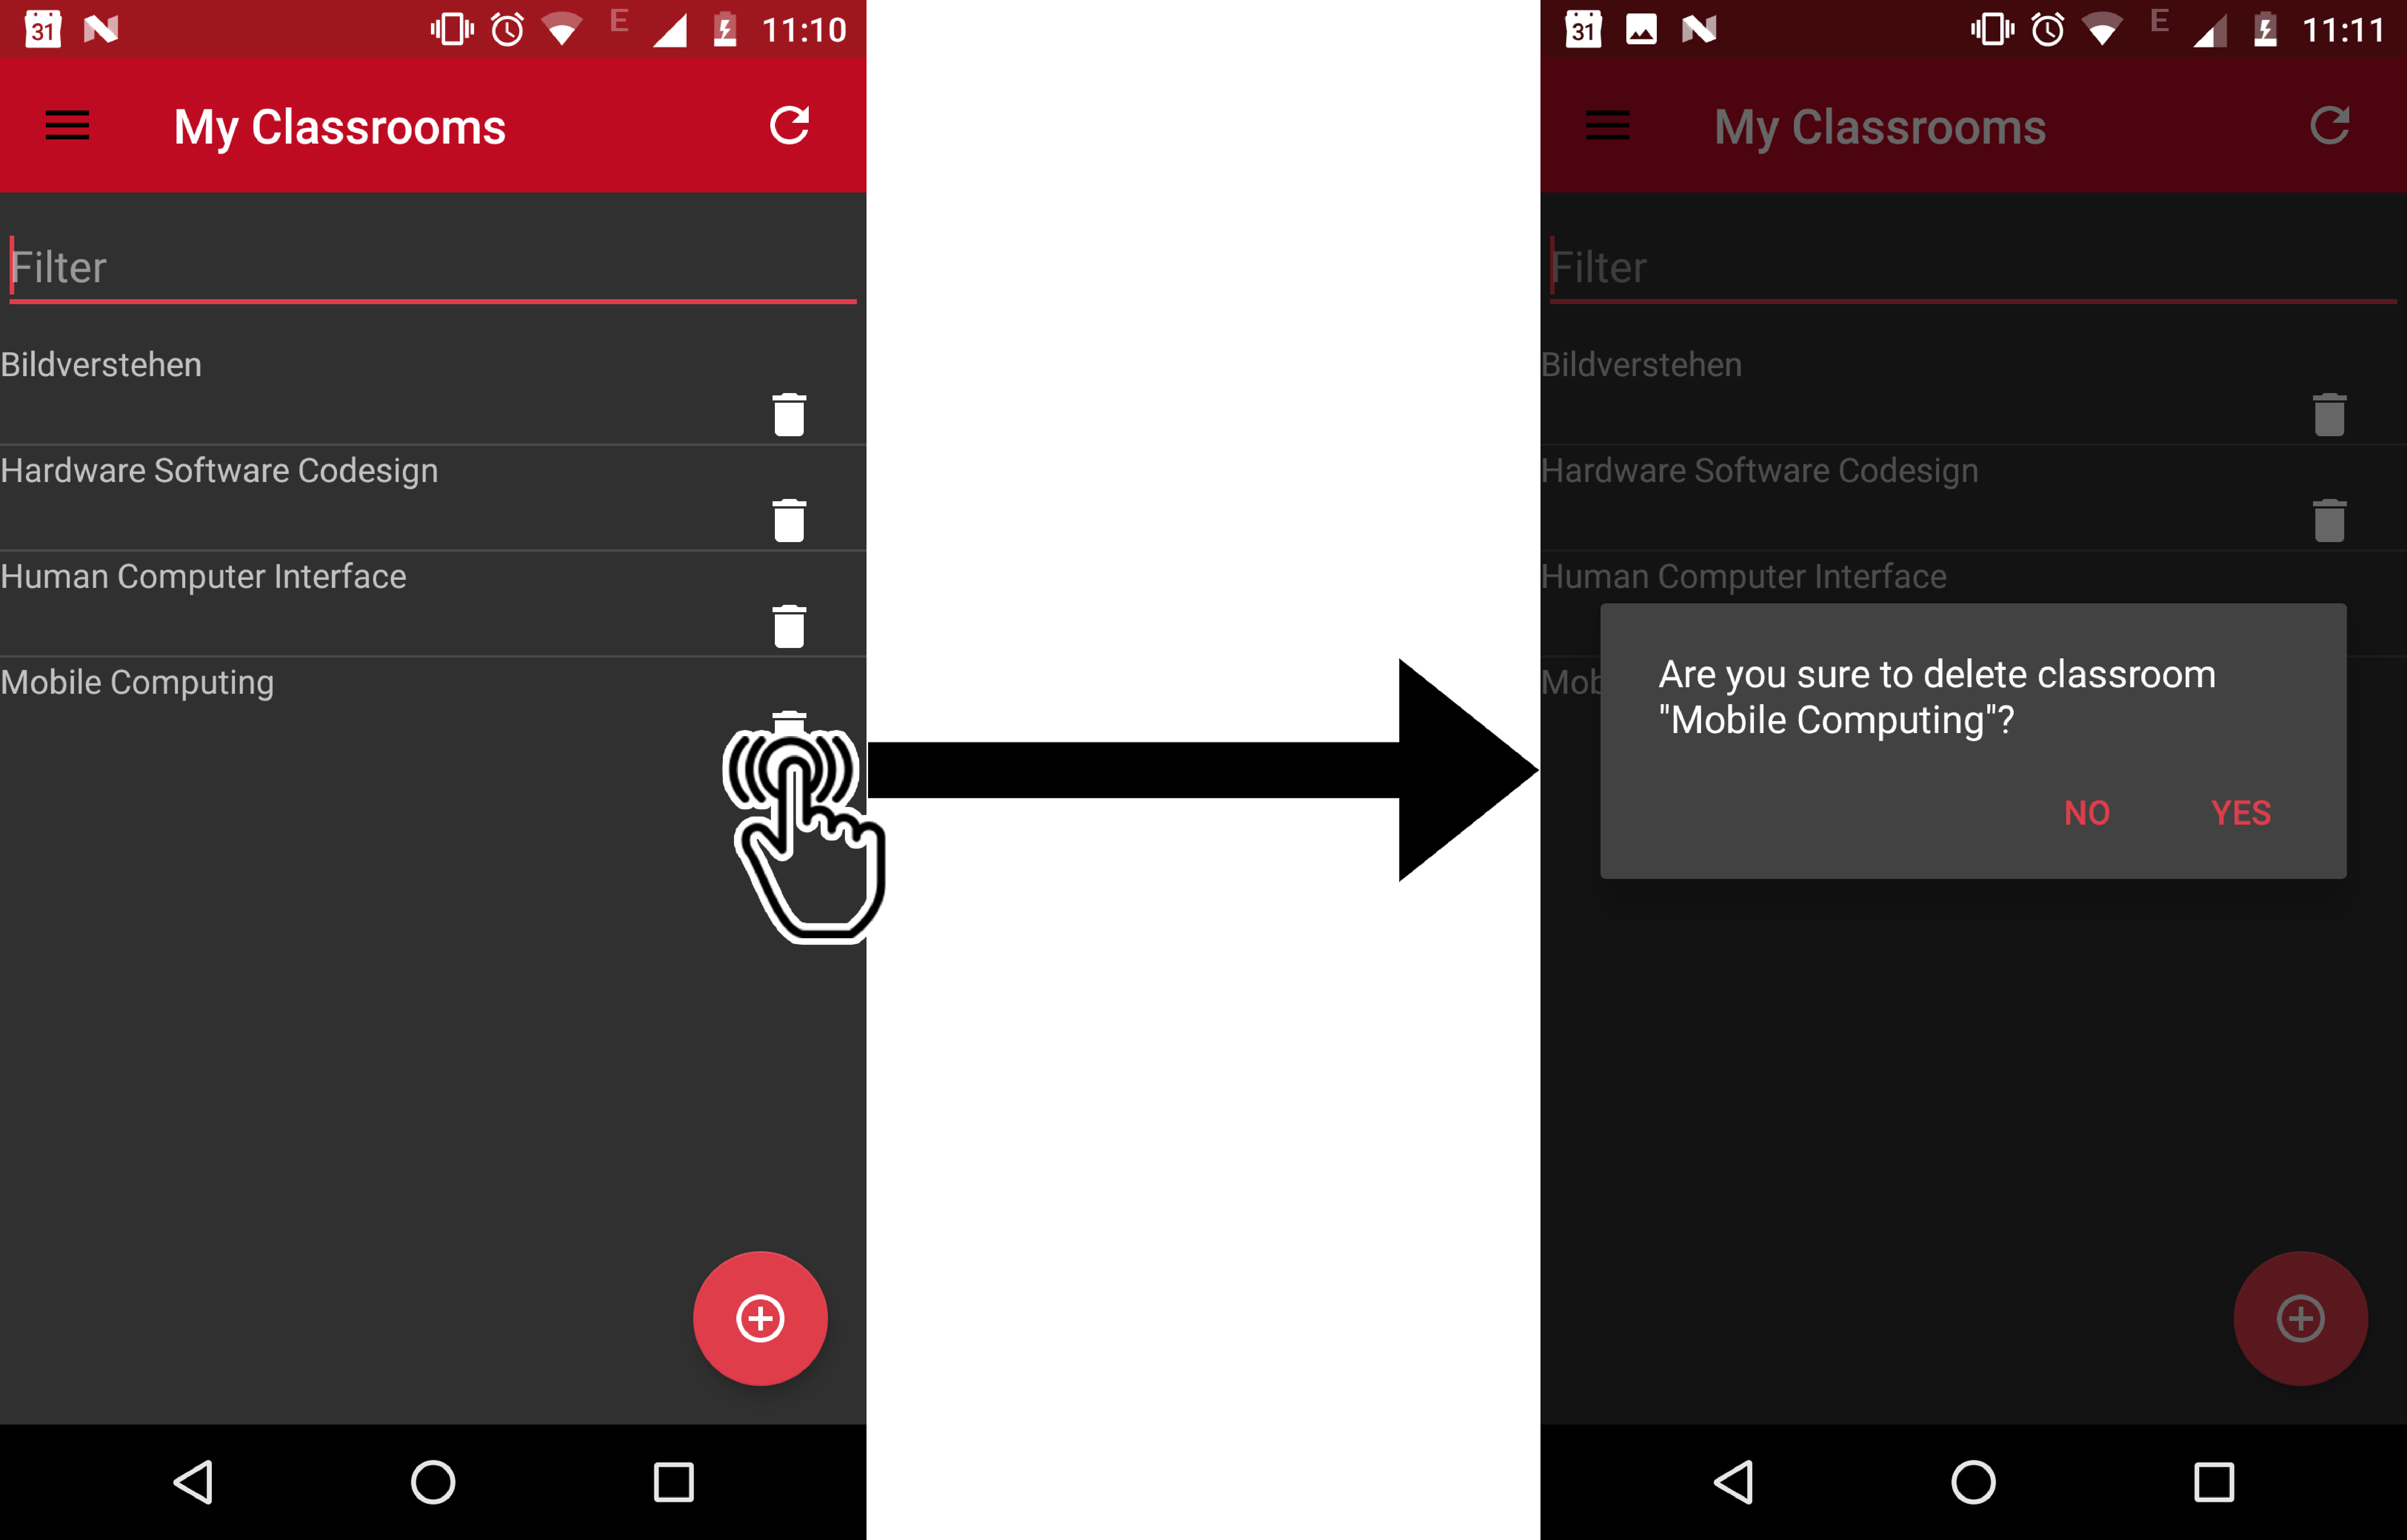
\includegraphics[scale=0.10]{Resources/LecturerMyClassrooms}
	\caption{Löschen eines Kursraums für Benutzer in der Rolle \enquote{Dozent}}
	\label{pic:LecturerDeleteClassroom}
	\end{center}
\end{figure}

\begin{figure}[H]
	\begin{center}
	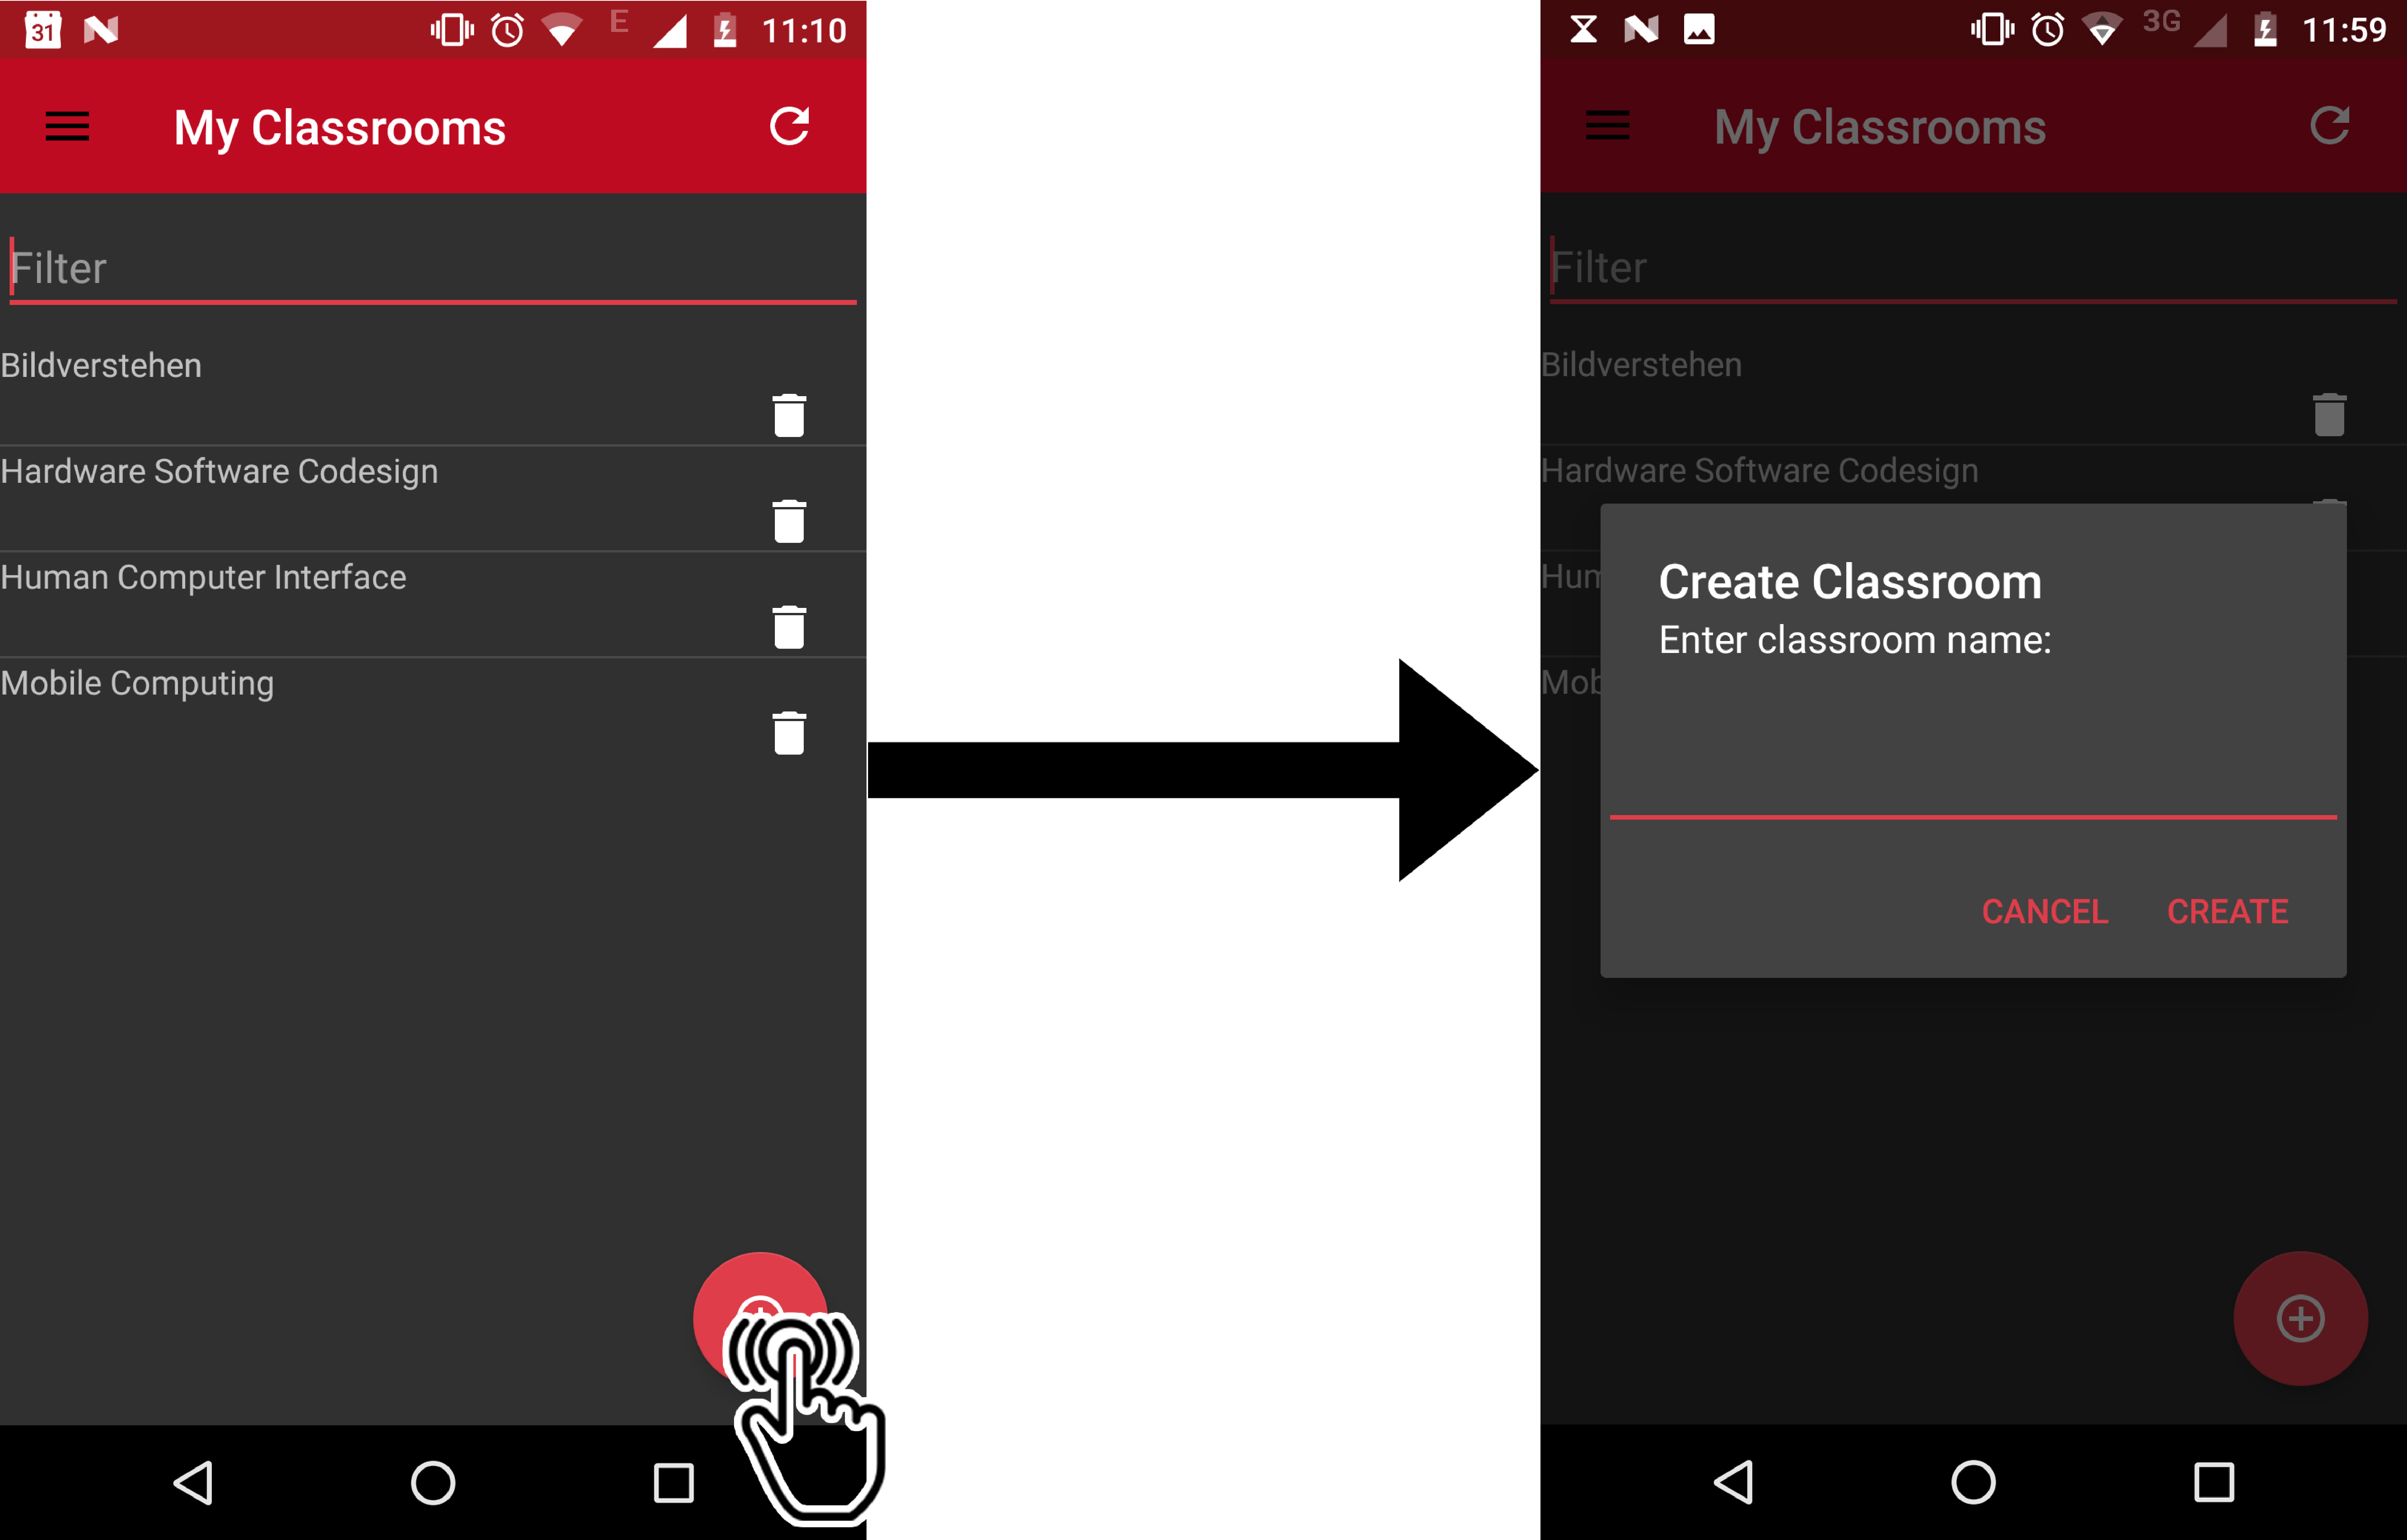
\includegraphics[scale=0.10]{Resources/LecturerCreateClassroom}
	\caption{Erstellen eines Kursraums in der Rolle \enquote{Dozent}}
	\label{pic:LecturerCreateClassroom}
	\end{center}
\end{figure}

Durch Klicken auf den Namen eines Kursraums wird in die Übersichtansicht für den gewählten Kursraum 
(siehe Abbildung \ref{pic:LecturerClassroom}).
Es werden nun alle Nachrichten angezeigt, die der Dozent in der Vergangenheit in den Kursraum eingestellt hat.
Nun besteht die Möglichkeit eine neue Nachricht zu erstellen.
Hierfür muss der \enquote{erstellen}-Button in der Ansicht unten rechts gedrückt werden.
Nun erscheint ein Dialog, in dem der Inhalt der neuen Nachricht eingegeben werden kann.
Mit \enquote{Okay} wird das Erstellen der Nachricht bestätigt; sie ist nun für alle Studenten, die diesen Kursraum abonniert haben sichtbar.
Für genaueres Verständnis ist der Ablauf dieser Benutzerinteraktion in Abbildung \ref{pic:LecturerPostMessage} dargestellt.
Möchte der Dozent eine Nachricht aus dem Kursraum entfernen, so betätigt er den \enquote{Löschen} Button neben der betreffenden Nachricht. 
Nun erscheint ein Dialog, der den Benutzer zu erneutem Bestätigten der Löschung aufruft.
Bestätigt der Anwender mit der Option \enquote{Delete} so wird die Nachricht gelöscht.
\begin{figure}[H]
	\begin{center}
	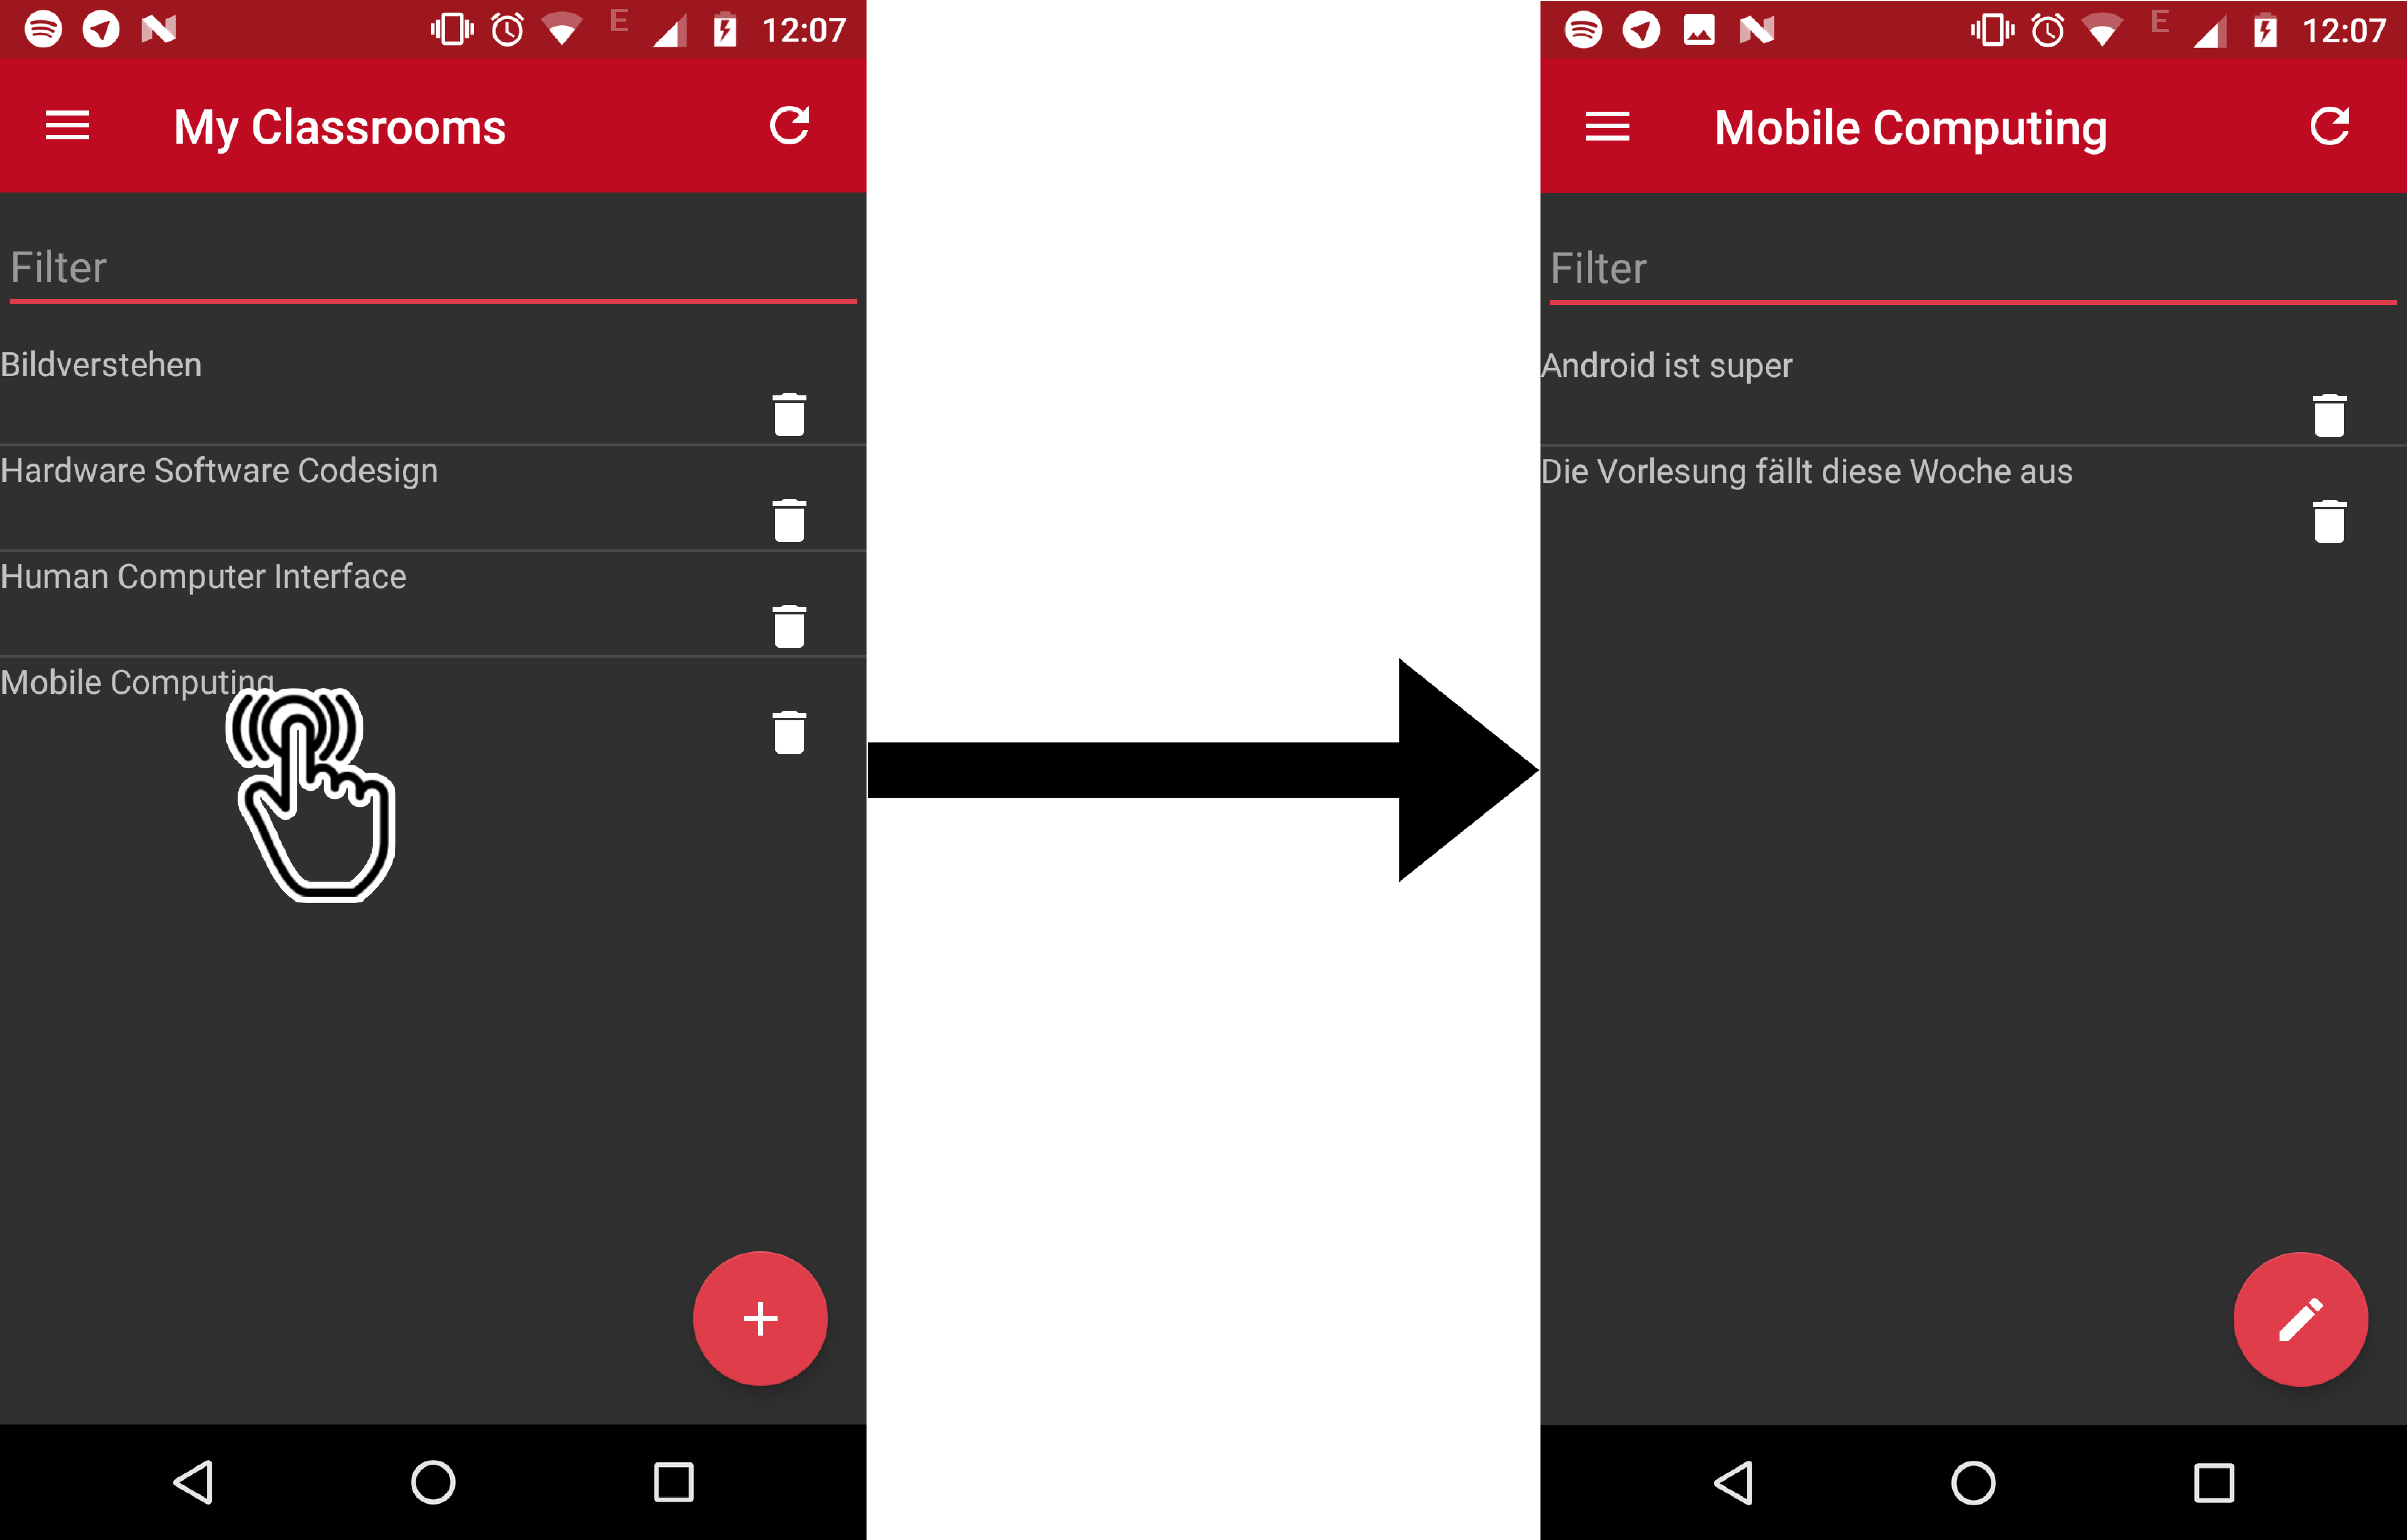
\includegraphics[scale=0.10]{Resources/LecturerClassroom}
	\caption{Wechseln zur Übersicht über einen Kursraum für Benutzer in der Rolle \enquote{Dozent}}
	\label{pic:LecturerClassroom}
	\end{center}
\end{figure}

\begin{figure}[H]
	\begin{center}
	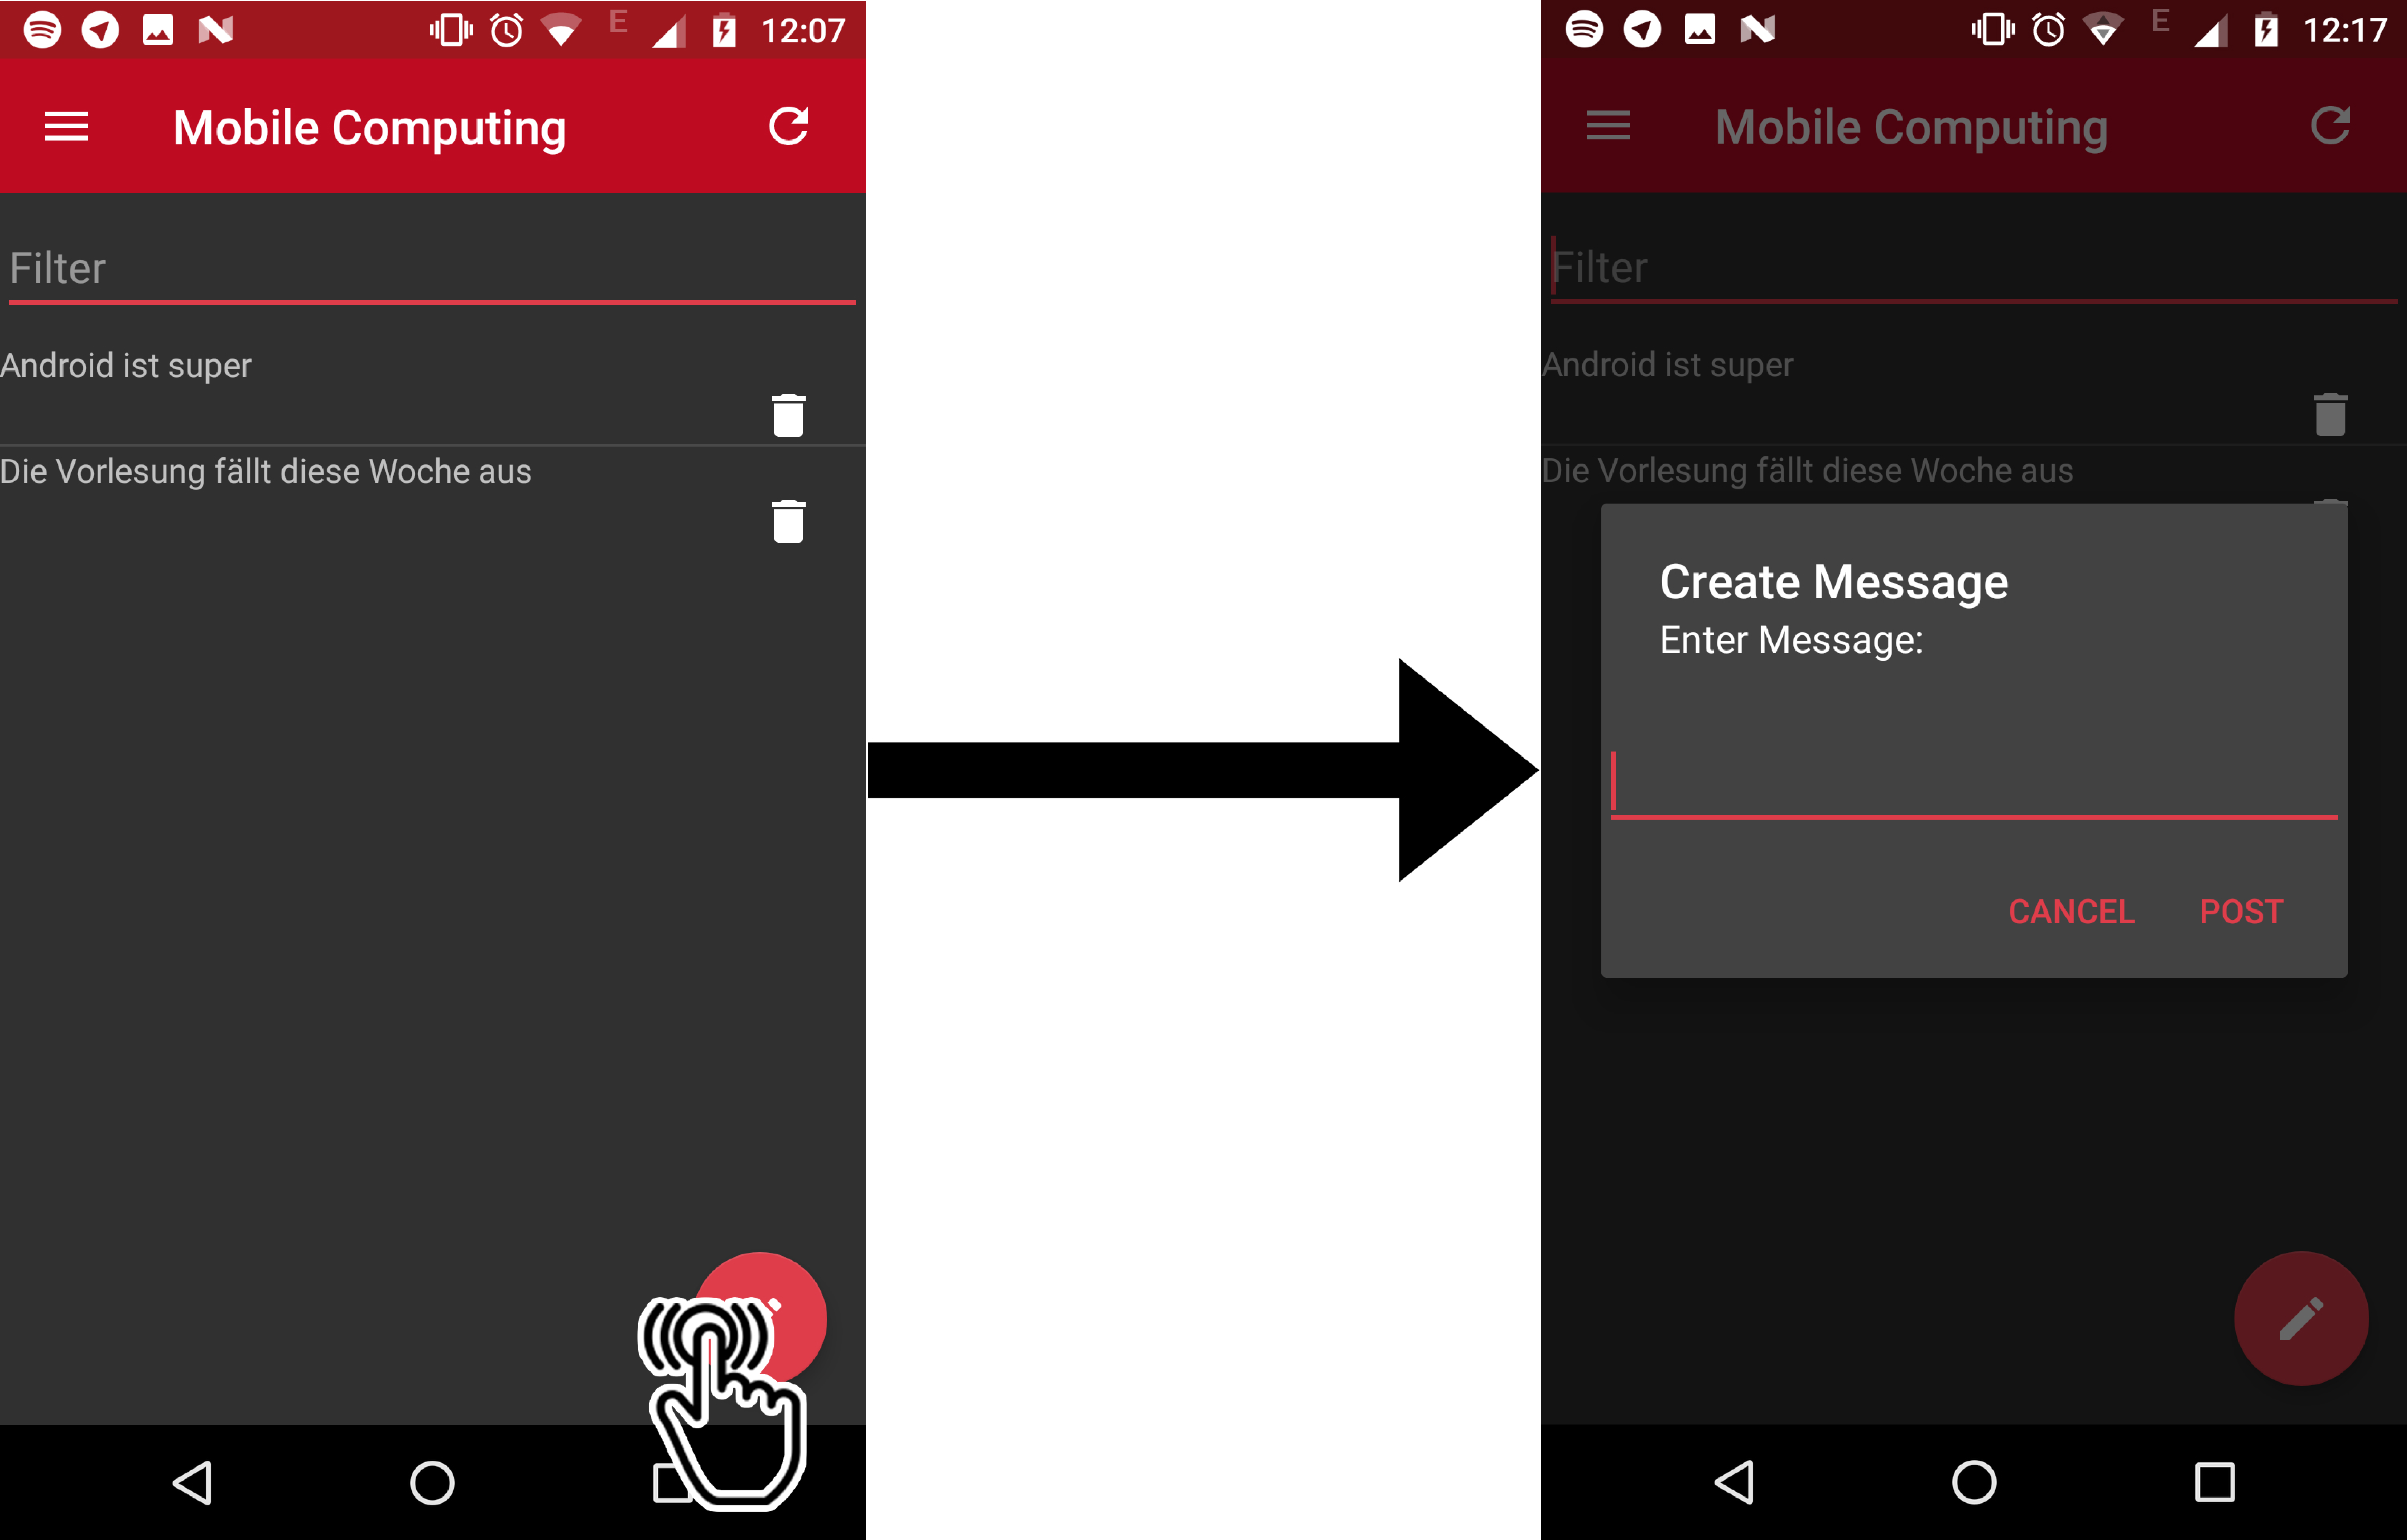
\includegraphics[scale=0.10]{Resources/LecturerPostMessage}
	\caption{Einstellen einer Nachricht in einem Kursraum für Benutzer in der Rolle \enquote{Dozent}}
	\label{pic:LecturerPostMessage}
	\end{center}
\end{figure}

\begin{figure}[H]
	\begin{center}
	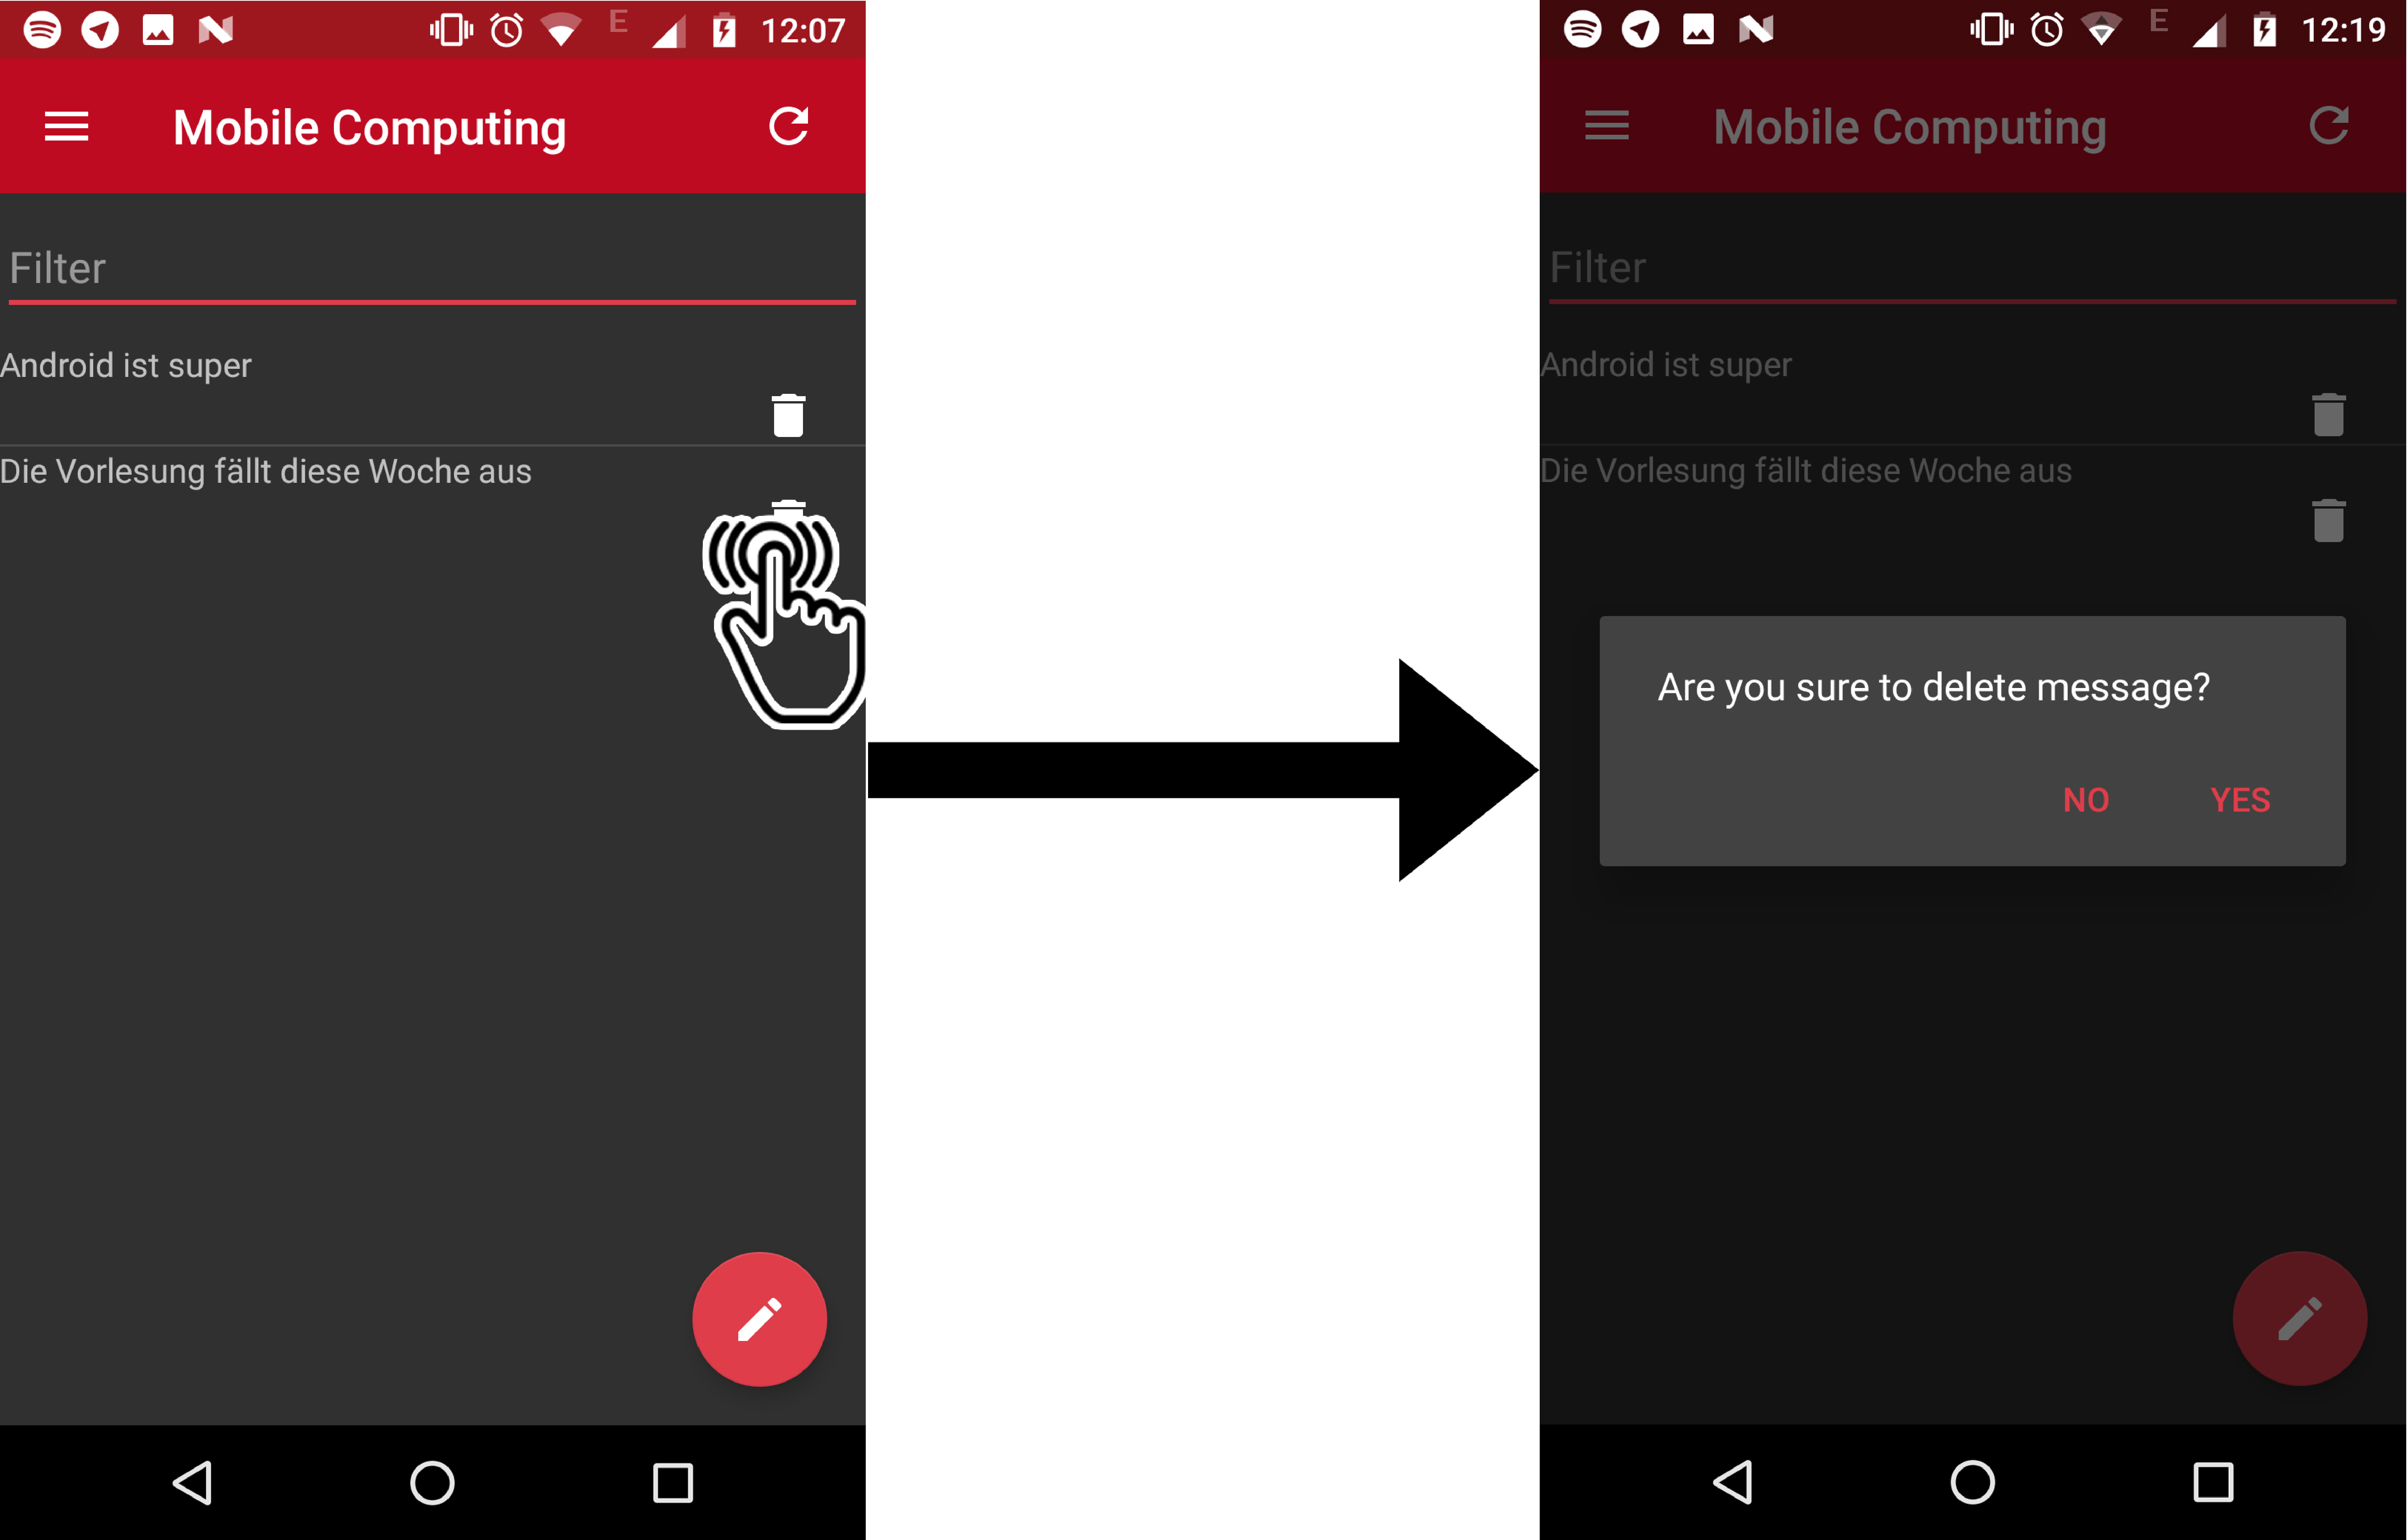
\includegraphics[scale=0.10]{Resources/LecturerDeleteMessage}
	\caption{Löschen einer Nachricht in einem Kursraum für Benutzer in der Rolle \enquote{Dozent}}
	\label{pic:LecturerDeleteMessage}
	\end{center}
\end{figure}



\newpage
\section{Oberfläche für Studenten}\label{section:StudentenOberflache}
Nach erfolgreicher Anmeldung wird einem Studenten die Oberfläche aus Abbildung \ref{pic:StudentenMyMessages} gezeigt. Hier werden alle Nachrichten aus seinen abonnierten Kursräumen -- sortiert nach Einstellzeitpunkt -- angezeigt.
Die angezeigten Daten werden sofort nach betreten dieser Ansicht vom Server geladen.
Durch Drücken auf das \enquote{Refresh} Symbol oben rechts, werden die Nachrichten erneut vom Server abgerufen und eventuell zwischenzeitlich neu eingestellte ebenfalls angezeigt.
Der Menü-Button oben links führt den Benutzer in die Ansicht aus Abbildung \ref{pic:StudentenOberflache}.
Zur Verbesserung der Übersichtlichkeit kann in dem Texteingabefeld \enquote{Filter} ein Suchtext eingegeben werden; es werden so nur noch Nachrichten angezeigt, deren Kursraum oder Nachrichtentext die eingegebene Zeichenfolge enthält.
\begin{figure}[H]
	\begin{center}
	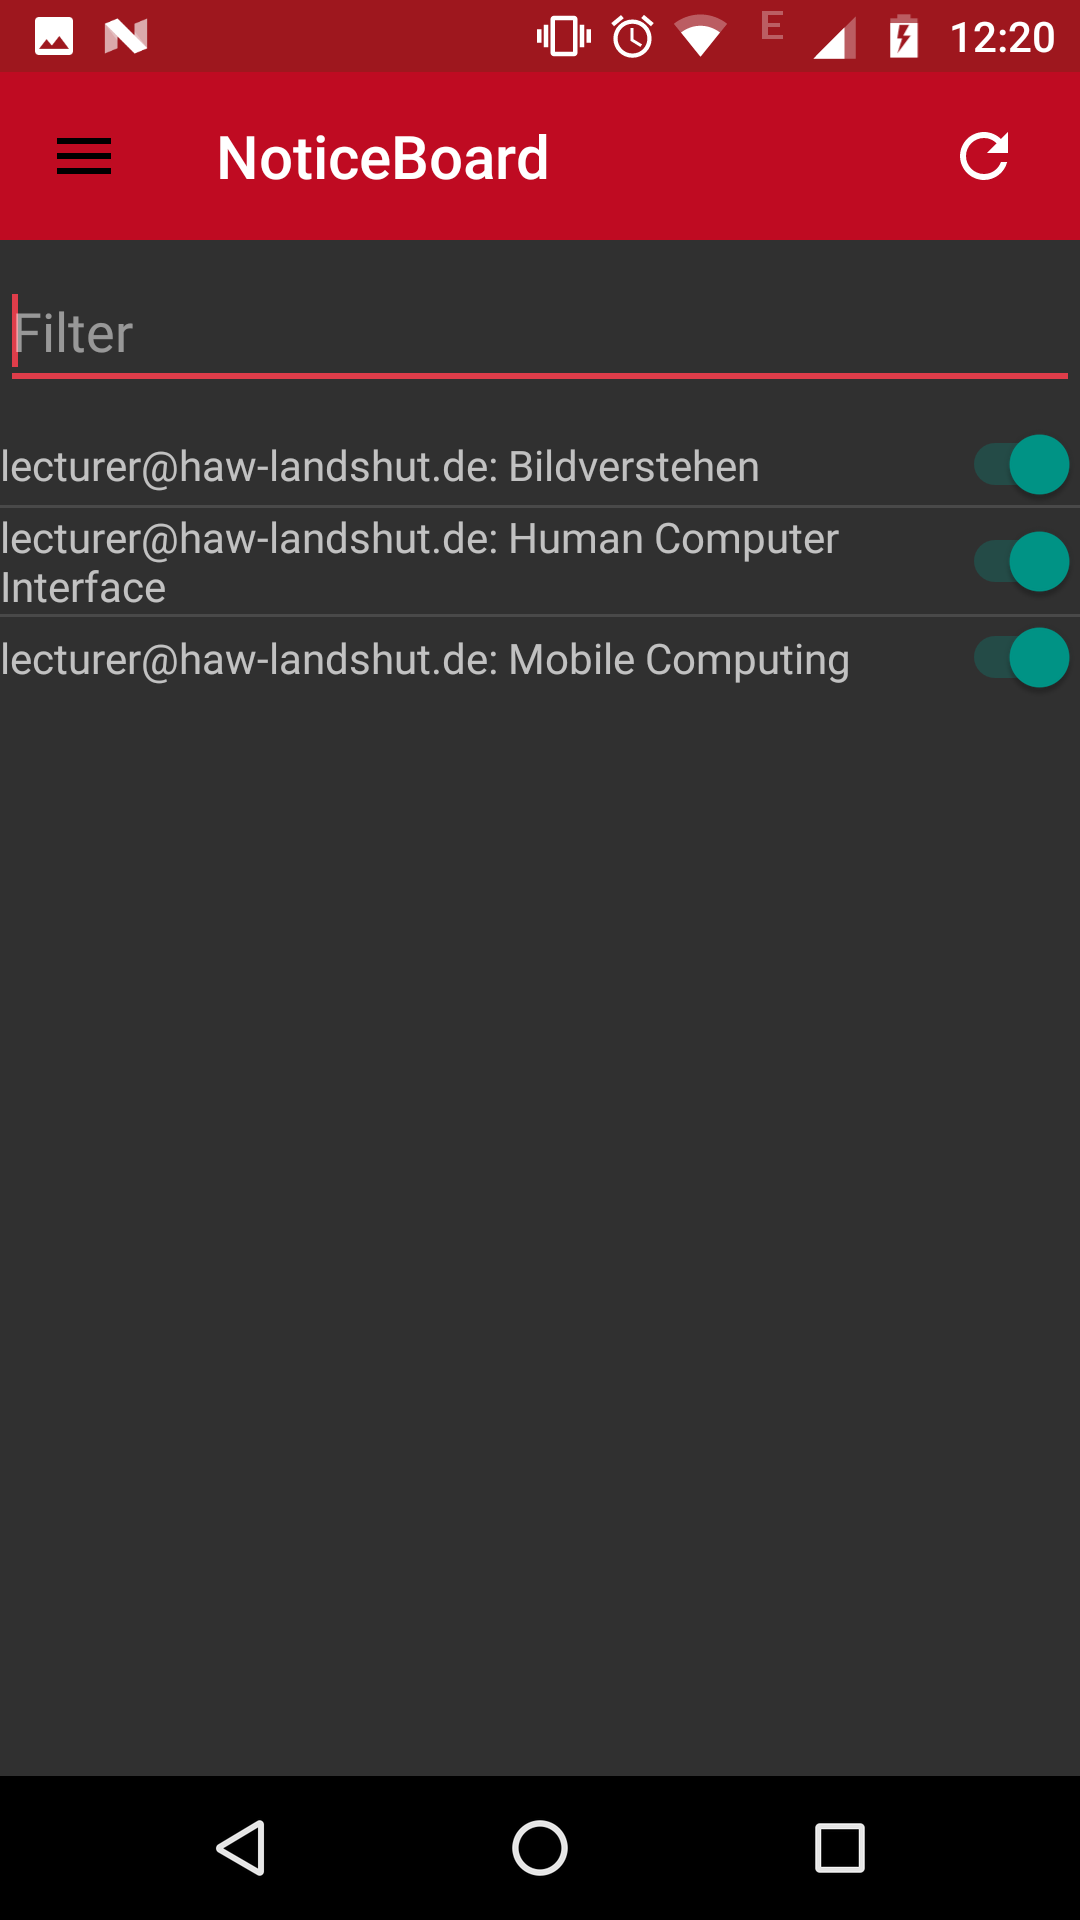
\includegraphics[scale=0.1]{Resources/ActivityMyClassrooms}
	\caption{Hauptmenü für Benutzer in der Rolle \enquote{Student}}
	\label{pic:StudentenMyMessages}
	\end{center}
\end{figure}

Studenten können mittels des in Abbildung \ref{pic:StudentenOberflache} gezeigtem Screens durch die App navigieren.
Es können mit \enquote{My Messages} alle aktuellen Nachrichten der abonnierten Kursräume angezeigt werden. 
Unter \enquote{My Classrooms} werden alle abonnierten Klassenräume geladen, diese können hier deabonniert werden.
Über die Option \enquote{All Classrooms} werden alle offenen Kursräume angezeigt; ein Student hat so die Möglichkeit diese zu abonnieren beziehungsweise zu deabonnieren.
Über den Menüpunkt \enquote{logout} meldet sich der Anwender aus der Applikation ab und gelangt zurück in die Authentifizierungsansicht.
\begin{figure}[H]
	\begin{center}
	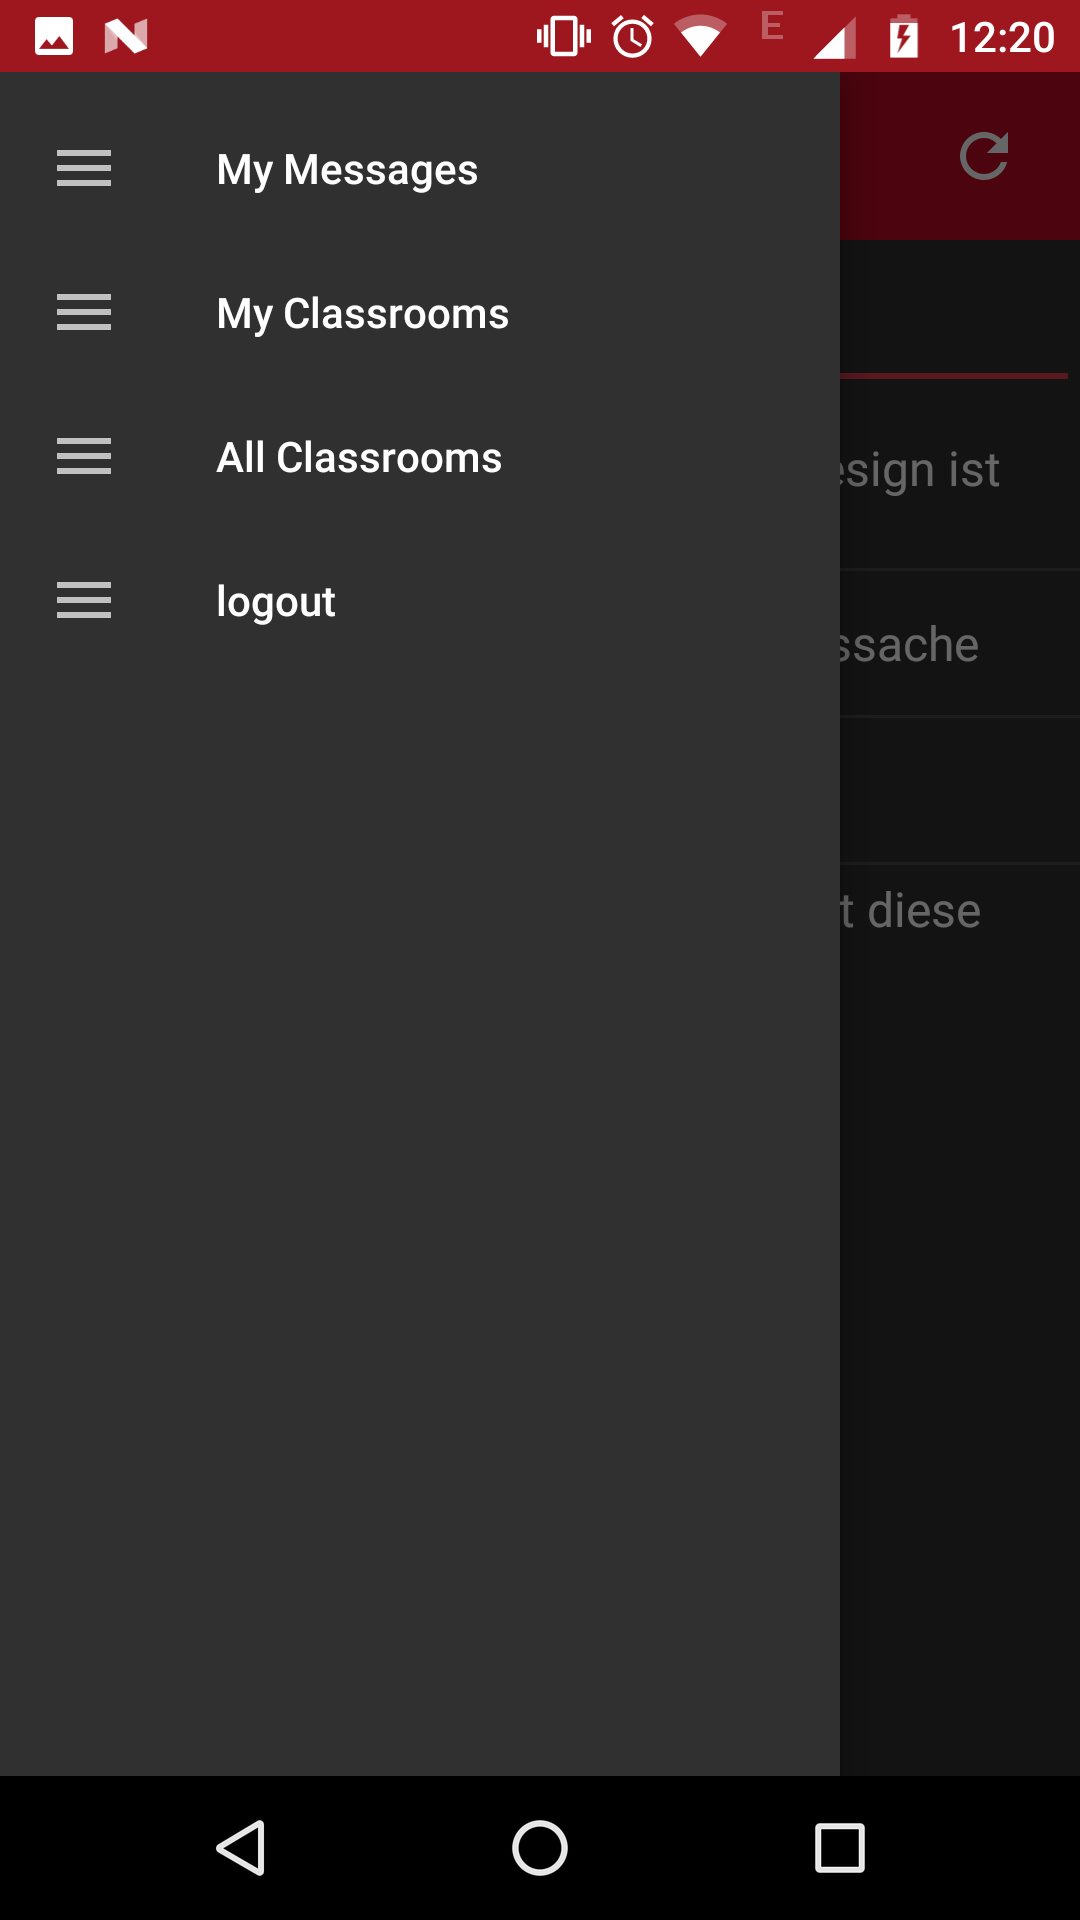
\includegraphics[scale=0.10]{Resources/ActivityMainMenuStudent}
	\caption{Hauptmenü für Benutzer in der Rolle \enquote{Student}}
	\label{pic:StudentenOberflache}
	\end{center}
\end{figure}
\newpage
In der Ansicht, die in Abbildung \ref{pic:StudentenMyClassrooms} dargestellt ist, werden Benutzern in der Rolle \enquote{Student} alle Kursräume und der zugeordnete Dozent angezeigt, die sie abonniert haben.
Rechts neben jedem abonnierten Kursraum befindet sich ein Schalter, der anzeigt, ob der betreffende Klassenraum abonniert ist oder nicht. 
Bei Betreten der Ansicht werden alle Kursräume als abonniert markiert. 
Durch Betätigen des Schalters wird der entsprechende Kursraum deabonniert und der Schalter steht auf aus. 
Es besteht die Möglichkeit durch erneutes Drücken den Kursraum wieder zu abonnieren; erst bei manueller Aktualisierung mittels des \enquote{Refresh}-Symbols wird der Kursraum entfernt. 
Filtern analog zur Oben beschriebenen Oberfläche ist ebenfalls möglich.
\begin{figure}[H]
	\begin{center}
	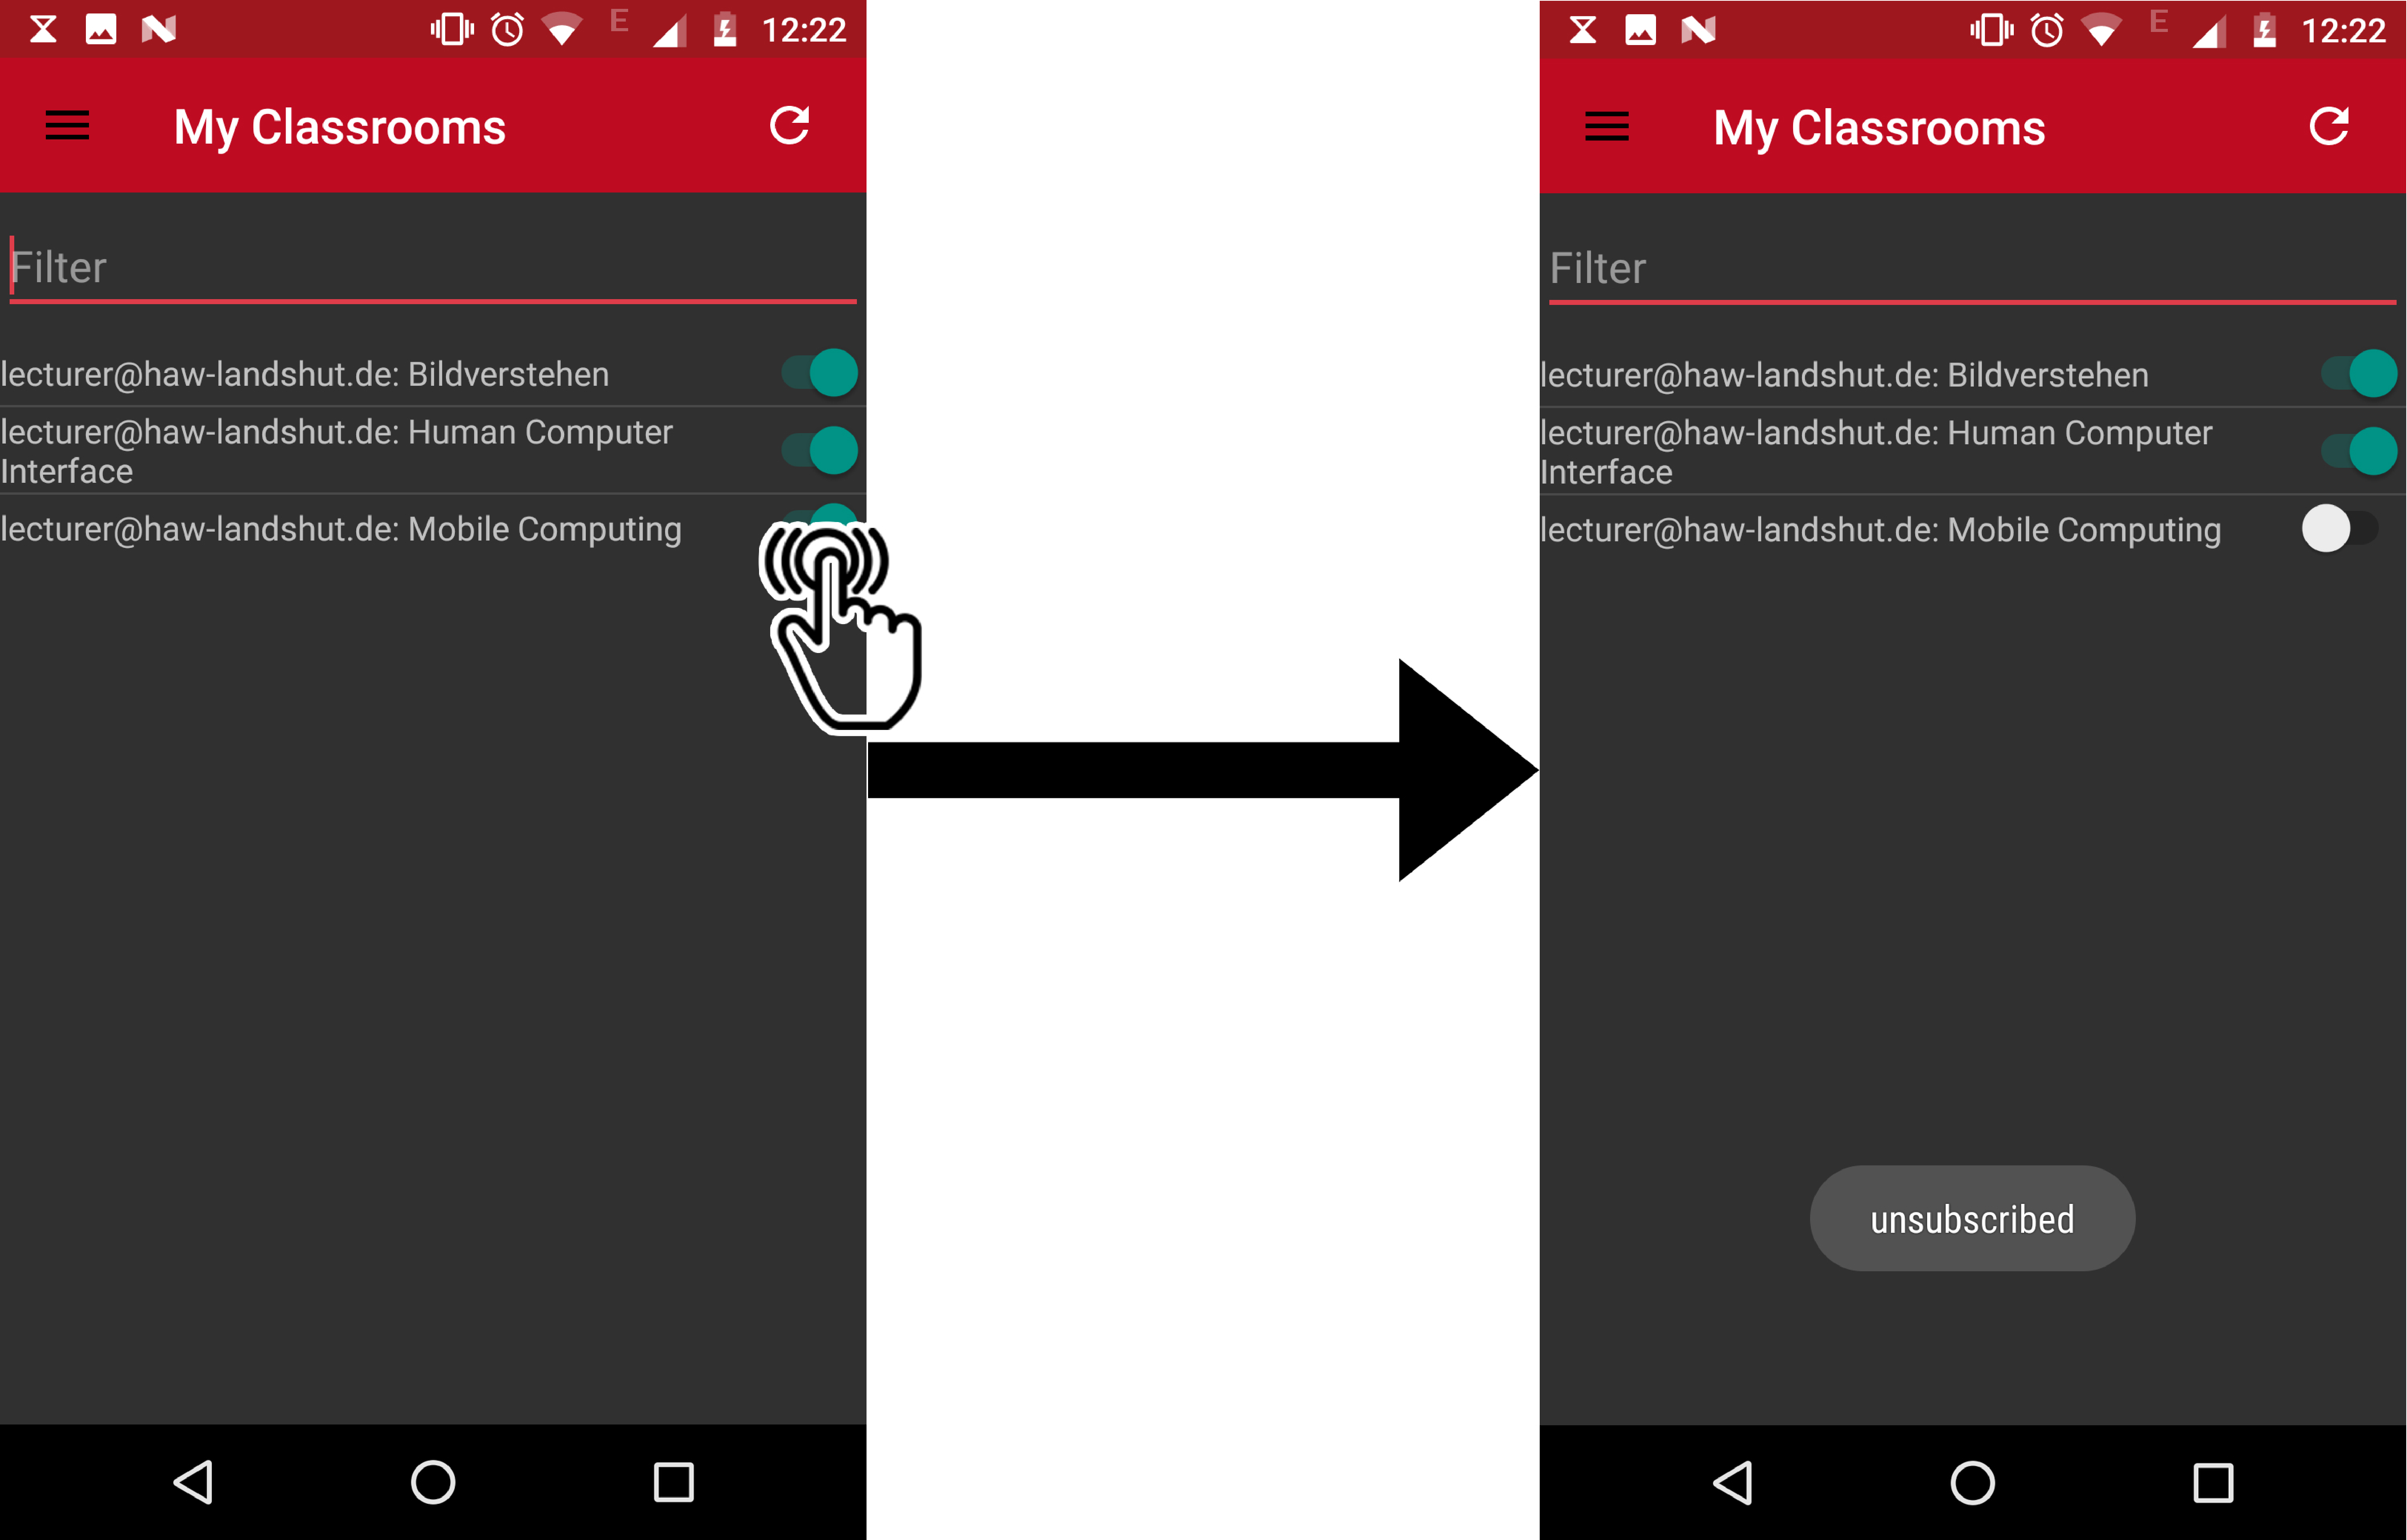
\includegraphics[scale=0.10]{Resources/StudentUnsubscribeClassroom}
	\caption{Deabonnieren eines Kursraums für Benutzer in der Rolle \enquote{Student}}
	\label{pic:StudentenMyClassrooms}
	\end{center}
\end{figure}

Die Activity \enquote{All Classrooms} (Abbildung \ref{pic:StudentenAllClassrooms}) zeigt alle Kursräume, die vom Benutzer abonniert werden können. Nicht abonnierte Kursräume werden mit einem deaktiviertem Schalter markiert und umgekehrt.
Der Anwender hat hier die Möglichkeit weitere Kursräume zu suchen und abonnieren oder gegebenenfalls auch zu de-abonnieren.
Bei Betreten dieser Activity werden die aktuellen Daten vom Server abgerufen, Betätigen des \enquote{Refresh}-Symbols aktualisiert die Daten manuell.
Über das Menü Symbol gelangt der Benutzer zurück in die Navigation.
\begin{figure}[H]
	\begin{center}
	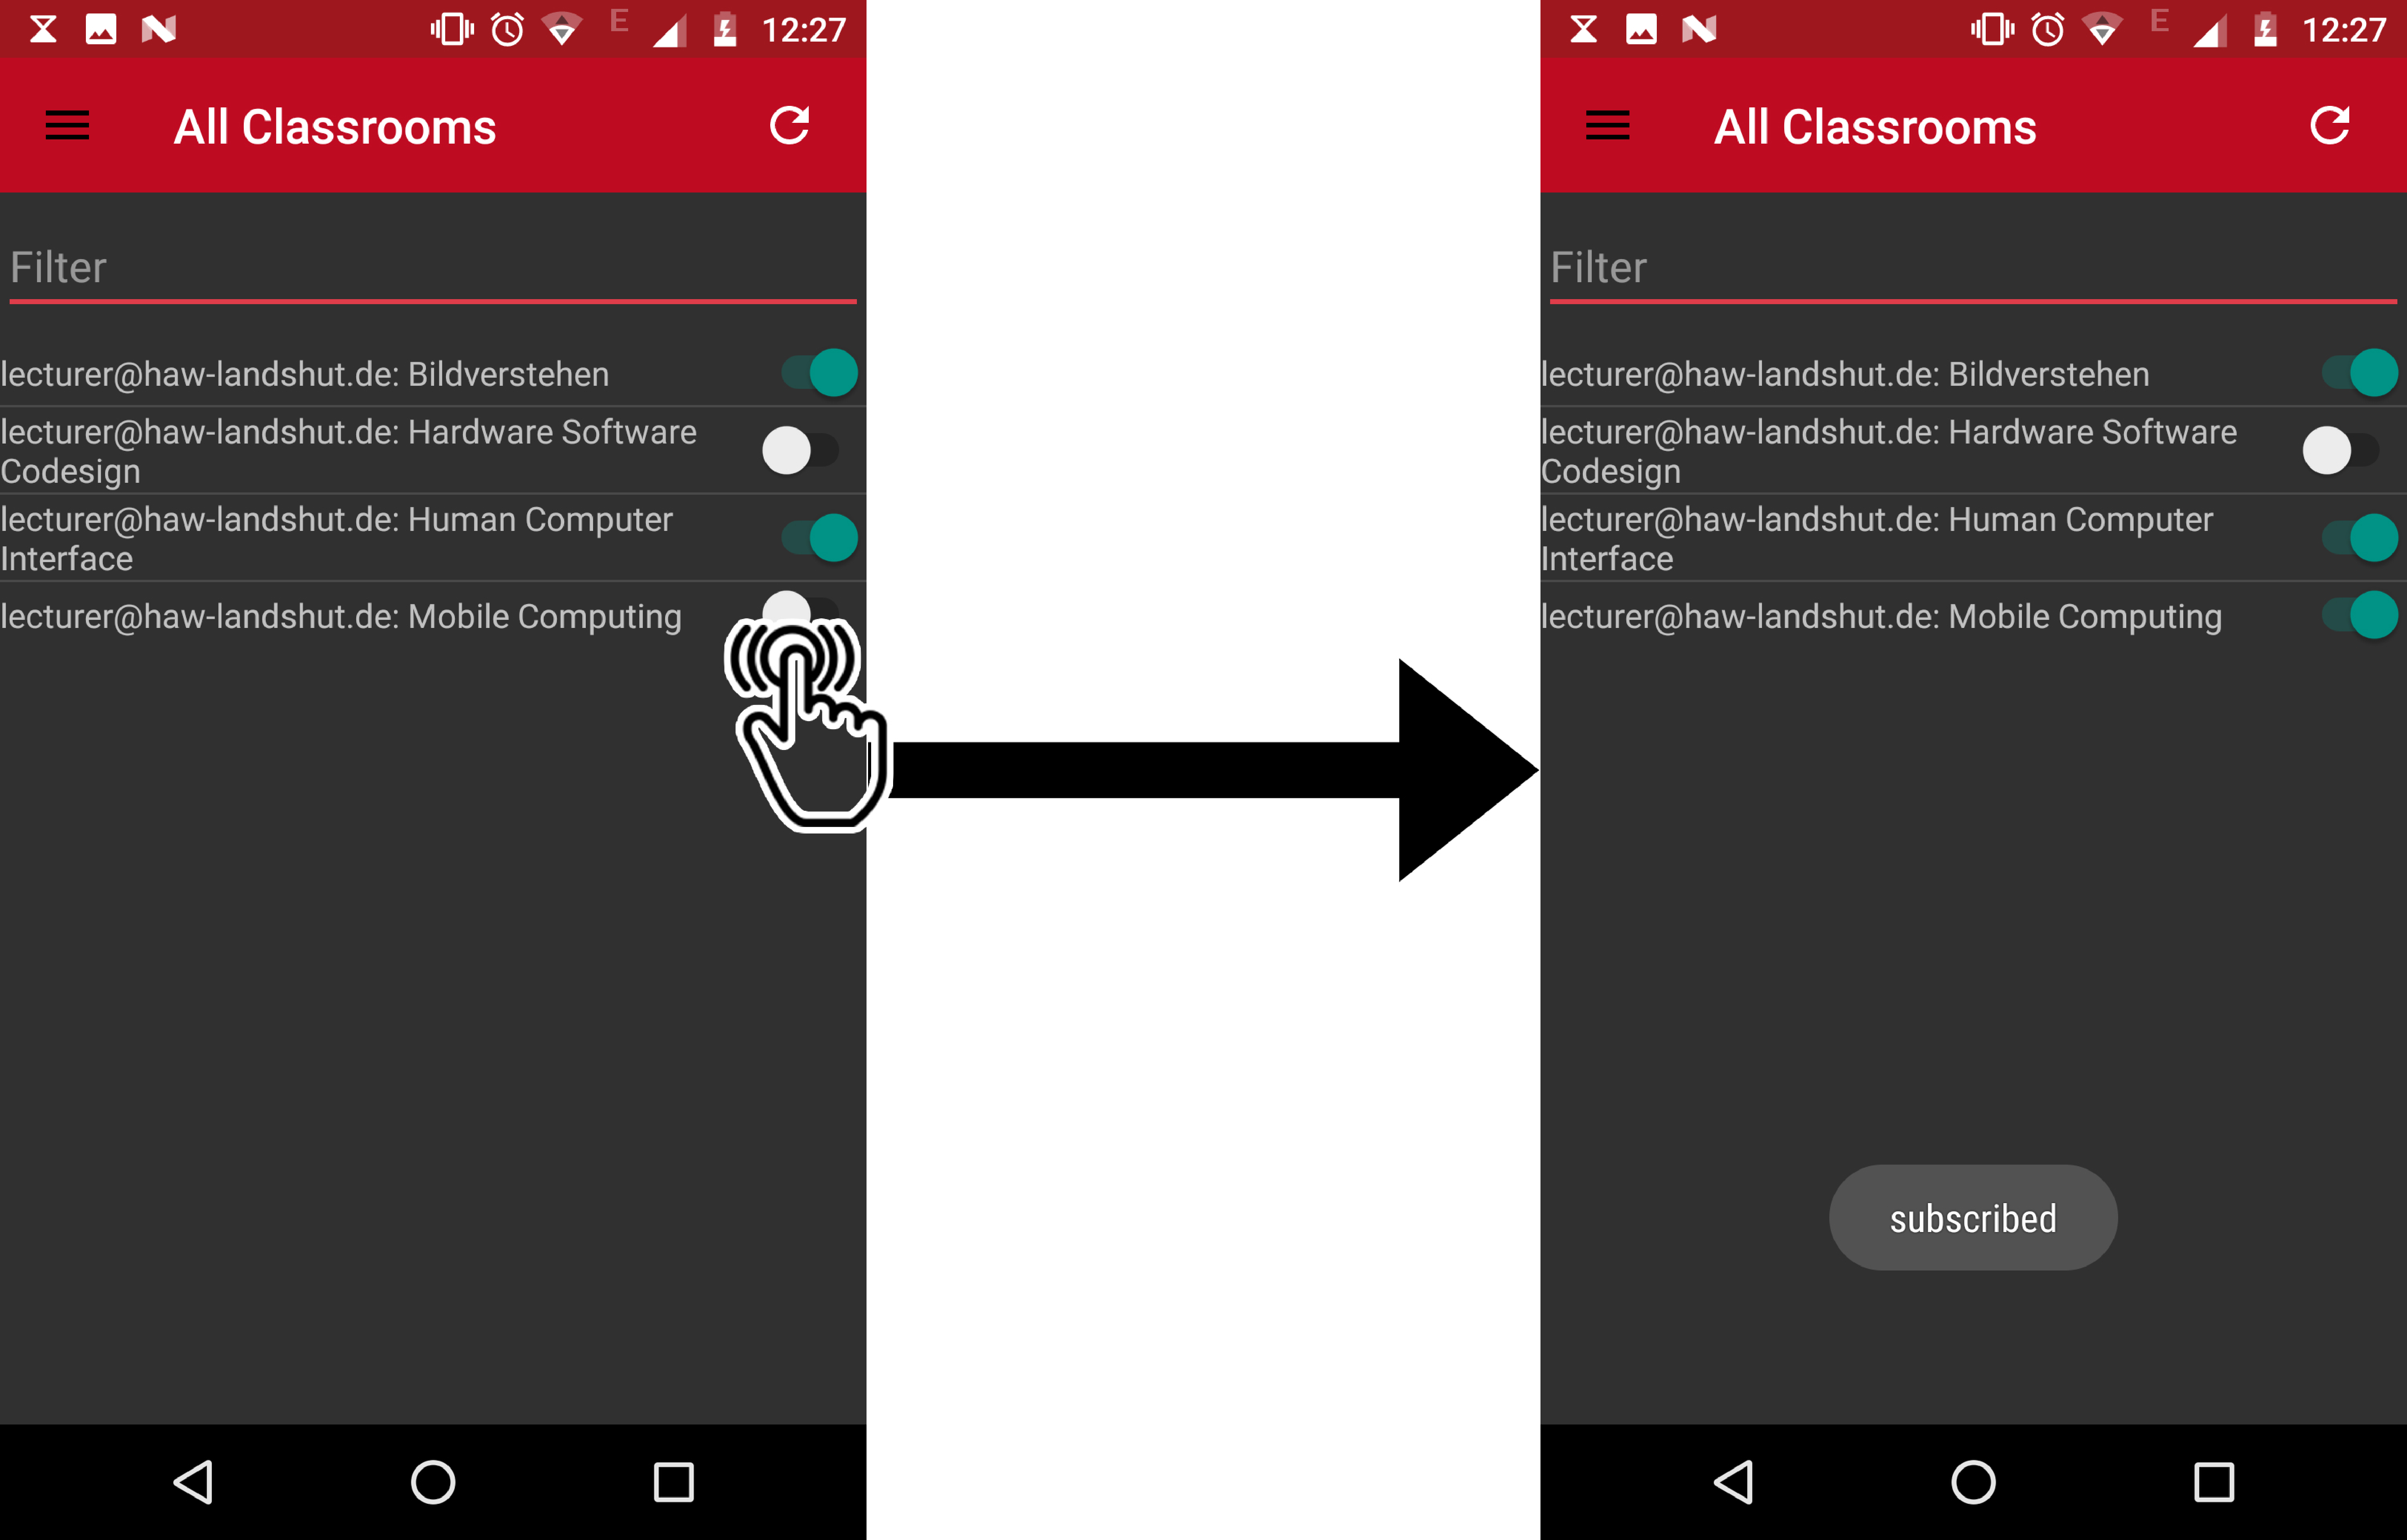
\includegraphics[scale=0.10]{Resources/StudentSubscribeClassroom}
	\caption{Abonnieren eines Kursraums für Benutzer in der Rolle \enquote{Student}}
	\label{pic:StudentenAllClassrooms}
	\end{center}
\end{figure}